\documentclass[12pt]{article}
\usepackage[margin=1in]{geometry}
\usepackage{longtable}
\usepackage{bm}
\usepackage{hyperref}
\hypersetup{
    colorlinks=true,
    linkcolor=black,
    filecolor=magenta,
    urlcolor=red,
    citecolor=cyan
}
\usepackage{graphicx}
\usepackage{rotating}
\usepackage{amsmath}
\usepackage{setspace}
\usepackage{amssymb}
\usepackage{natbib}
\usepackage{amsfonts}
\usepackage[table]{xcolor}
\usepackage{booktabs}
\usepackage{subcaption}
\usepackage{courier}

\newcommand\citeapos[1]{\citeauthor{#1}'s (\citeyear{#1})}
\newcommand{\R}{\texttt{R}} % Write R in typewriter font

\begin{document}

\title{The Network of Foreign Direct Investment Flows: \\Theory and Empirical Analysis}
\author{John  Schoeneman\thanks{\footnotesize{
PhD Student, Pennsylvania State University, jbs5686@psu.edu.}} \and Boliang Zhu\thanks{\footnotesize{Assistant Professor, Department of Political Science, Pennsylvania State University, bxz14@psu.edu. }} \and Bruce A. Desmarais\thanks{\footnotesize{Associate Professor, Department of Political Science, Pennsylvania State University, bdesmarais@psu.edu}}}
\date{}
\maketitle

\singlespacing
\begin{abstract}
    \noindent We study the structure of the international network of foreign direct investment (FDI) flows. The political economy of FDI literature has established several theoretical claims and empirical regularities regarding exogenous political and economic determinants of FDI inflows. %These include security alliances, preferential trade agreements, migration networks, and colonial history.
    However, existing studies---based on monadic and to a lesser degree, dyadic regression models---overlook the complex dependencies that are likely to characterize the network. Recent developments in methodology for studying international relations show that the regression framework is typically inadequate for quantitatively modeling dyadic relational data, such as FDI flows. In this paper, we integrate hypotheses regarding exogenous determinants and novel hypotheses regarding structural dependencies into a comprehensive exponential random graph model (ERGM) for weighted networks. Our findings reveal that the FDI flow network  exhibits a number of complex dependencies, such as reciprocity and transitivity, that have been omitted from previous empirical models of FDI flows.

\end{abstract}

\clearpage
\doublespacing
\section{Introduction}


What accounts for the pattern of global foreign direct investment (FDI) flows? Scholars have long been interested in understanding the determinants of FDI flows across countries. Standard economic models attribute cross-border capital movements primarily to relative factor endowments, market size, and transportation and trade cost \citep[see,~e.g.,][]{Helpman:1984,Carr_et_al:2001}. Yet, footloose capital becomes immobile ex post and thus an ``obsolescent bargain,'' which is vulnerable to host government's expropriation \citep{Vernon:1971,Vernon:1980}. Building on this insight, the recent political economy of FDI literature emphasizes the importance of political institutions in constraining host government's opportunistic behavior. Scholars suggest that political constraints \citep{Henisz:2000}, democratic governance \citep{Jensen:2003,Jensen:2006}, rule of law \citep{Li_Resnick:2003,Staats_Biglaiser:2012}, and signing in international trade and investment agreements \citep{Buthe_Milner:2008,Allee_Peinhardt:2011} help to ensure policy credibility and provide investor protection, thereby luring in foreign investors.

To date, existing theories have focused exclusively on firm-level characteristics and home- and host-country economic and political parameters to explain cross-border FDI flows. The literature implicitly assumes that FDI flows into one country or between a dyad are independent of each other. This assumption, nonetheless, unlikely holds, given the intertwined links among multinational corporations (MNCs) and the expansion of global production networks \citep{UNCTAD:2013}. If global FDI flows can arise endogenously from the network structure, existing political economy models of FDI remain incomplete by excluding high-order structural variables. Furthermore, neglecting network structure variables may lead to biased estimates or even invalid inferences \citep{cranmer2011inferential}.

We argue that two network structures---reciprocity and transitivity---are important to explain the pattern of cross-border FDI flows. First, reciprocity arises from the fact that FDI represents an oligopolistic expansion strategy of MNCs and the fact that host governments tend to use a principle of reciprocity to regulate FDI inflows. Second, the expansion of global supply chains and the diffuse of preferential trade agreements (PTAs) drive the transitivity/clustering of investment activities, leading to network dependencies.

To test our arguments, we use the count exponential random graph model (ERGM) to account for network dependencies in a standard gravity model of FDI inflows. Utilizing bilateral FDI flow data from United Nations Conference on Trade and Development (UNCTAD) over the period of 2001--2012, we find strong evidence that FDI inflows are reciprocal and transitive/clustering, suggesting that cross-border FDI flows are interdependent and shaped by their network structure. We also find that ignoring high-order network structure variables can lead to biased estimates of key explanatory variables such as destination polity and trade openness in standard panel regression models.

The paper proceeds as follows. Next section discusses the independent assumptions in the study of FDI, and international relations in general. Following that, we theorize the reciprocity and transitivity of FDI inflows and present testable hypothesis. After that, we discuss the research design and present empirical results. Finally, the paper concludes.



%Research examining foreign direct investment (FDI) and its relationship with economic and political determinants is expansive. Much of this work is conducted using the gravity model, which was originally developed to predict trade flows. This framework models FDI flows using dyadic data and the product of partner GDPs as mass and some variant of distance as an independent variable. Our work highlights a key weakness of these models that rely on standard panel regression models. There has been a growing body of literature that brings into question the way we estimate models for dyadic data. The primary challenge is that dyadic data is an edge-list and therefore represents a network. Ignoring this unmodeled network structure violates assumptions within a generalized linear model, particularly independence, potentially leading to biased estimates. While there is a growing body of work that has addressed the interdependence problem in dyadic data, especially for trade, FDI has been largely ignored. We address this gap in the literature through the use of network modeling to test previous theories alongside of estimating dependence terms.


%{\bf [John or Boliang, paragraph on what scholars have asked or know about FDI]}



\section{Independence Assumptions and the Study of FDI}

The dominant eclectic paradigm suggests that MNCs arise from taking advantage of firms' intangible or specific assets to overcome imperfections in arm's length transactions \citep{Caves:1996,Dunning:1992}. In this sense, direct investment or the establishment of foreign affiliates is a decision made by a parent company. The recent political economy of FDI literature starts with the premise that footloose capital becomes relatively immobile after investment takes place, and thus a hostage to host government \citep{Vernon:1971,Vernon:1980}. MNCs are ex post vulnerable to host government's opportunistic behavior such as asset expropriation or even subtle policy changes that dampen firms' profitability. Adopting a neo-institutionalist approach, scholars emphasize the role of domestic and international institutions in preventing state's predatory behavior and ensuring credible commitment, thereby attracting FDI \citep[e.g.][]{Henisz:2000,Jensen:2003,Jensen:2006,Li_Resnick:2003,Staats_Biglaiser:2012,Buthe_Milner:2008,Allee_Peinhardt:2011}

There is now a large empirical literature examining the determinants of FDI inflows \citep[e.g.,][]{Noorbakhsh_et_al:2001,Yeaple:2003,Jensen:2003,Li_Resnick:2003,Buthe_Milner:2008,Li_Vashchilko:2010,Kerner:2009}. Existing studies typically model FDI flows at the monadic and to a lesser extent at the dyadic level. One implicit assumption in existing theoretical and empirical models is that FDI flows into one country or between a dyad are independent of other countries or dyads. However, given the complex inter and intra-firm relationships and the expansion of global production networks \citep{UNCTAD:2013}, we expect that high-order network structures should play a critical role in shaping the pattern of FDI flows.

% Paragraph on interdependence in IR/IPE
Historically, statistical models used in international relations have involved the implicit assumption that countries and dyads are independent of each other \citep{diehl2016conditional,ward2007persistent}. This assumption is now widely viewed as dubious \citep[see, e.g., ][]{ward2007persistent, chu2010homogenization,cranmer2016critique,dorff2013networks,lee2013network,howell2013geography,kinne2016agreeing}. The negative consequences of erroneously assuming independence are two-fold. First, the model is misspecified, which leads to biased estimates and hypothesis tests for covariates included in the model. Second, researchers arrive at a limited theoretical scope in which they only consider the relationship between the dependent variable and covariates, and do not consider the influences that relationships and countries have on each other. The methodological toolkit available to scholars of international relations has advanced well beyond conventional regression approaches, and now offers at least three prominent options for modeling interdependence in relational data----stochastic actor oriented models \citep[e.g., ][]{camber2010geometry,kinne2016agreeing,kinne2013network,kinne2014dependent,warren2016modeling}, exponential random graph models \citep[e.g.,][]{cranmer2012complex,cranmer2012toward,raeymaeckers2016influence}, and latent space models \citep[e.g., ][]{ward2007disputes,ward2013gravity,metternich2013antigovernment}. As such, it is quite methodologically feasible to move beyond questionable independence assumptions in the study of FDI.


\section{Dependence Hypotheses in FDI Flows}



\subsection{Reciprocity of FDI Flows}
Reciprocity stems from the fact that FDI represents an oligopolistic expansion strategy of MNCs \citep{Hymer:1976,Kindleberger:1969}. MNCs arise from exploiting their ownership-specific assets to overcome imperfections in arm's-length markets \citep{Caves:1996,Dunning:1992}. These proprietary assets include, for instance, advanced technology, brand names, product differentiation, and managerial and advertising skills, which are of a public-goods character and possess substantial economies of scale. To make the most use of these firm-specific assets and best exploit economies of scale, MNCs actively seek to expand into each other's home markets. Unsurprisingly, until the first decade of the new century, FDI flows mainly between developed countries, especially among the triad of the European Union, Japan, and the United States.

MNCs' oligopolistic expansion often encounters opposition from host government due to concerns of national security, market monopoly, and protection of indigenous firms. In order to gain access to foreign markets, MNCs have incentives to leverage their influence on home government for reciprocity \citep{Milner:1988,Crystal:2003}. As \citet[6]{Crystal:2003} note, ``they [MNCs] want to counter the existing restrictions---on both trade and FDI---that some foreign countries have imposed and so therefore will favor contingently restrictive policies.'' \citet{Tingley:2015}, for instance, show that U.S. government officials are more likely to oppose Chinese firms' mergers and acquisitions when China has blocked U.S. investment.

We also expect that the degree of reciprocity varies by host countries' levels of development. Investing abroad incurs large fixed costs and firms need to overcome the disadvantages such as ``liability of foreignness'' they face when competing with indigenous firms in the host country. Therefore, only the most productive firms are able to engage in FDI activities \citep{Melitz:2003,Helpman_et_al:2004}. Historically, MNCs from developed countries predominate. In the past two decades, FDI from developing and transition economies have grown rapidly. Yet developing-country MNCs still account for a relatively small share of global outward FDI. For instance, in 2005 outward FDI flows and stocks from developing countries are approximately 17\% and 13\% of the world total, respectively \citep{UNCTAD:2006}. Furthermore, outward FDI from developing countries is highly concentrated; the top 10 countries, mostly large emerging economies such as Argentina, Brazil, Chile, China, Mexico, Russia, and South Africa contribute about 83\% \citep{UNCTAD:2006}. Firms in most developing countries are still technologically backward and not competitive enough to thrive in a global market. Thus, we hypothesize the following:

\textit{Hypothesis 1: FDI flows are likely to be reciprocal.}

\textit{Hypothesis 1a: The reciprocity of FDI flows is stronger among developed dyads than others.}

\subsection{Transitivity/Clustering of FDI Flows}
Two factors are likely to drive the transitivity/clustering of investment activities---the expansion of global supply chains and the diffuse of PTAs.  One distinct feature of today's globalization is the increasing fragmentation of production processes and the dramatic expansion of global supply chains \citep{UNCTAD:2013}. At the center of global production networks are MNCs, which coordinate global supply chains through complex networks of their foreign affiliates, subcontractors, or arm's-length suppliers \citep[xxii]{UNCTAD:2013}. These intertwined networks give rise to the clustering of FDI activities. In a most straightforward way, MNCs' establishment of a foreign affiliate can result in investment of their partners such as upstream suppliers or downstream purchasers, who themselves are often multinationals that coordinate their own networks of supply chains. This kind of interdependence leads to multiple triangle closures of investment flows. Consider a case of three countries: A, B, and C. Firms from A invest in B as suppliers to firms in B.\footnote{Alternatively, firms in A can export intermediate goods to B. However, firms typically favor near suppliers. Moreover, if transportation and trade costs between A and B are high, firms in A will prefer direct investment over export \citep{Carr_et_al:2001}. } If these downstream firms in B establish foreign affiliates in C to exploit locational advantages such as a large consumer market or favorable government policies, investment by upstream firms in A likely follows to serve these foreign affiliates. For instance, Volkswagen's investment in Skoda Auto in Czech Republic not only attracted other auto makers such as PSA Peugeot and Toyota, but also international suppliers of parts and components to acquire local firms or build new factories; ``As of 2002, there were 270 firms operating in the Czech Republic, representing 45 percent of the top 100 world suppliers of automotive parts and components.'' \citep[352]{Kaminski_Javorcik:2005}. 

More importantly, global supply chains tie countries together and significantly increase the cost of government's opportunistic behavior---such as expropriation or subtle policy changes---that deters foreign investment. Investors' wariness stems from the fact that footloose capital becomes an ``obsolescent bargain'' given its ex post immobility, and thus a hostage to the host government \citep{Vernon:1971,Vernon:1980}. Global production networks significantly constraint government's policy discretion, because the proper functioning of the supply chains hinges crucially on the cooperation and coordination of countries involved. For example, even Starbucks, a company that has a relatively simple supply chain, ``sources coffee from thousands of traders, agents and contract farmers across the developing world; manufactures coffee in over 30 plants, ...; distributes the coffee to retail outlets through over 50 major central and regional warehouses and distribution centres; and operates some 17,000 retail stores in over 50 countries across the globe'' \citep[142]{UNCTAD:2013}.

Apparently, any interruption in the global supply chain can severely damage Starbucks's business. Thus, governments are incentivized to refrain from arbitrary interventions or even subtle policy changes that jeopardize their position in global production networks. Especially when countries are integrated into the same global production network, the risk-mitigating effect of the network is magnified because involving countries have strong incentives to ensure the well-functioning of the network, which their prosperity depends on. As \citet{Kim_Solingen:2017} show, East Asian countries that are integrated into global production networks are more likely to promote cooperation and peace between each other. Therefore, we expect that FDI has a higher probability than a random chance to flow among countries that are in the same global production network, resulting in the clustering of investment activities.

In addition, the diffuse of PTAs is likely to drive the clustering of direct investment activities as well. The formation of a PTA eliminates trade barriers among member states. The removal of trade barriers allows MNCs to optimize their global supply chains and fragment its production stages within member states to best capitalize on locational advantages such as factor endowments and favorable government policies. For instance, with the increasing integration of the European Community, the 1980s witnessed a restructuring of many industries and regionalization of MNC activities to exploit the advantages of a single market, leading to a surge of intra-region FDI \citep[34]{UNCTAD:1991}. Importantly, most favored-nation treatment, investment clauses, and dispute-settle mechanisms that are embedded in PTAs help to alleviate foreign investors' concerns of government interventions, discrimination, and expropriation \citep{Buthe_Milner:2008,buthe2014foreign}, thereby making member states more attractive investment destinations to each other. PTAs therefore reinforce the clustering of investment activities.

\textit{Hypothesis 2: FDI flows are likely to be transitive/clustering.}






\section{Data and Research Design}


We estimate a gravity model of FDI flows. The dependent variable is bilateral FDI inflows. The data are from UNCTAD, covering the time-period of 2001 to 2012. The data set was first made available in 2014 \citep{UNCTAD:2014}. Most existing empirical studies on FDI use monadic data because scholars are primarily interested in how host countries' economic and political parameters affect capital inflows.\footnote{There are very few studies that use dyadic FDI data. See \citet{Frenkel_et_al:2004}, \citet{Li_Vashchilko:2010}, and \citet{Razin_et_al:2005}. } The advantage of using dyadic data is that it allows us not only to model network relationships, but to measure changes in FDI inflows related to covariates that are at the dyad level, such as PTAs, alliances, colonial history, and common language. To deal with the skewed distribution, we take the natural log of the bilateral FDI flow variable

\subsection{Covariates}

In the gravity model, we include the log product of the dyad's real GDP\footnote{The data comes from the \textit{Penn World Table}  \citep{feenstra2015next}.} and logged Euclidean distance.\footnote{See \citet{mayer2011notes} for the calculation of Euclidean distance.} Generally, larger products of GDP are associated with higher levels of FDI while longer distances are associated with less FDI. One key point here is that for the purpose of model convergence the logged product of dyadic GDP has been estimated as one variable in the model, rather than being estimated separately.

We also control for a country's trade openness (trade as \% of GDP) and GDP growth rate. Existing research has shown that FDI and trade are compliments \citep{aizenman2006fdi}. We expect that higher levels of trade openness will be associated with higher levels of FDI. High GDP growth rates stand in for the general health of a country's economy. Thus we expect that a high GDP growth rate to correlate with more FDI, both as a sender and receiver. Both data are from the World Bank's \textit{World Development Indicators}.

There is a substantial amount of work that explores the relationship between democratic institutions and FDI inflows; yet empirical results to date remain inconclusive \citep[see e.g.][]{Henisz:2000,Jensen:2003,Li_Resnick:2003,Jakobsen_DeSoysa:2006,Resnick:2001}. We include standard polity scores as a measure of a country's level of democracy \citep{Marshall_Jaggers:2010}. We also include political violence to proxy for state instability,\footnote{Data comes from \citet{marshall2005major}.} which should be negatively correlated with FDI inflows.

In addition, we include two sets of international agreement variables. The first is four dummy variables for different types of defense agreements, from \citet{Gibler09}. They include defense, entente, non-aggression, and neutrality treaties. We expect these variables to be positively associated with FDI inflows, particularly defense treaties since this indicates political cooperation and low political risk \citep{Li_Vashchilko:2010}. The second is preferential trade agreement (PTAs). Signing a PTA represents a commitment to liberal markets that investors would favor and therefore would be associated with increased FDI inflows \citep{Buthe_Milner:2008,buthe2014foreign}. Yet, PTAs vary significantly in depth with some requiring nearly full liberalization of trade barriers while others are superficial political signals. We thus measure the depth of PTAs by using latent trait analysis with 48 different dichotomous variables regarding topics covered in PTAs.\footnote{Data are from \citet{dur2014design}.}

\subsection{Model and Specification: The Count ERGM}

To model the FDI network, we must use a statistical modeling approach that is capable of representing the dependencies underlying the ties. The literature offers a number of options. These include the latent space family of models, such as those that have been used to model trade networks in political science \citep{ward2007persistent,ward2013gravity}; the generalized exponential random graph model (GERGM), which can be used to model complex network features in networks with continuous-valued edges \citep{desmarais2012statistical,wilson2017stochastic}; and the ERGM for count-valued edges \citep{krivitsky2012exponential}. We select the count-valued ERGM for two reasons. First, if the researcher's objective is to test hypotheses regarding dependent network structure, ERGM family models can accomplish this more precisely than can latent space models \citep{cranmer2016navigating,cranmer2016critique,desmarais2017statistical}. Second, the count ERGM offers a modeling advantage over the GERGM for data such as FDI flows, which are zero for the majority of dyads. That is, the count ERGM is capable of modeling zero inflation in the network. This paper presents, as far as we are aware, the first application in political science of the count ERGM proposed by \cite{krivitsky2012exponential}.

Like other forms of the ERGM, the count ERGM is a statistical model that operates on one or more network adjacency matrices. To specify the count ERGM, the researcher selects two types of network statistics---those that relate tie values to observed covariates (i.e., covariate effects), and those that relate the ties to each other via high order network structure (i.e., network effects). If an ERGM is specified without network effects, it reduces to a dyadic regression model in which ties are assumed to be independent and identically distributed \cite{cranmer2011inferential}. Under \citeapos{krivitsky2012exponential} count ERGM, the probability of the observed $n \times n$ network adjacency matrix $\bm{y}$ is $$ \text{Pr}_{\bm{\theta};h;\bm{g}}( \bm{Y}=\bm{y} )=\frac{ h(\bm{y})\text{exp}( \bm{\theta} \cdot \bm{g} (\bm{y}) )}{\bm{\kappa}_{h,\bm{g}}(\bm{\theta})},$$ where $\bm{g}( \bm{y} )$ is the vector of network statistics used to specify the model, $bm{\theta}$ is the vector of parameters that describes how those statistic values relate to the probability of observing the network, $h(\bm{y})$ is a reference function defined on the support of $\bm{y}$ and selected to affect the shape of the baseline distribution of dyadic data (e.g., Poisson reference measure), and $\bm{\kappa}_{h,\bm{g}}(\bm{\theta})$ is the normalizing constant that assures that the probabilities over all possible networks sums to one.


\subsubsection{Specification}


The count ERGM is extremely flexible in that there are very few constraints on the generative features that can be incorporated into the model through $\bm{g}( \bm{y} )$. In the models we specify, we use statistics that model the shape of the individual edge distributions (i.e., the shapes of directed dyadic FDI flows), model the dependencies we have described above, and account for the effects of exogenous covariates. The statistics we use to account for the individual edge distribution include, $$\text{Sum}:\bm{g(y)} = \sum_{(i,j) {\in} \mathbb{Y}}\bm{y}_{i,j},$$ which models the average edge value $$\text{Sum, Fractional Moment}:\bm{g(y)} = \sum_{(i,j) {\in} \mathbb{Y}}\bm{y}_{i,j}^{1/2},$$ which accounts for dispersion in the edge distribution, and
$$\text{Non-Zero}: \bm{g}_k = \sum_{(i,j) {\in} \mathbb{Y}} \mathbb{I}(\bm{y}_{i,j} \neq 0),$$ which models the prevalence of zeros in dyadic FDI flows. We include two statistics to model the dependencies that correspond to our hypotheses. First,
$$ \text{Reciprocity}: \bm{g(y)} = \sum_{(i,j) {\in} \mathbb{Y}}min(\bm{y}_{i,j},\bm{y}_{j,i}),$$ in which we add up the lowest edge value within each dyad. If edges are reciprocated, this statistic will increase due to the co-occurrence of large edge values within the same dyad. Second,
$$\text{Transitive Weights}: \bm{g(y)} =  \sum_{(i,j) {\in} \mathbb{Y}}\min\bigg( \bm{y}_{i,j}, \max\limits_{k{\in}N}\Big(\min(\bm{y}_{i,k},\bm{y}_{k,j})\Big) \bigg),$$ which acounts for the degree to which edge $(i,j)$ co-occurs with pairs of large edge values with which  edge $(i,j)$ forms a transitive (i.e., non-cyclical) triangle. Exogenous covariates are accounted for with statistics that measure the degree to which large covariate values co-occur with large edge values. First,
$$ \text{Dyadic Covariate}: \bm{g(y,x)} = \sum_{(i,j)} \bm{y}_{i,j}x_{i,j},$$ measures this co-occurrence at the level of the directed dyad, in which there is a dyadic observation of the covariate corresponding to each potential FDI flow. There are two statistics that account for node (i.e., country) level covariates. Each statistic takes the product of the node's covariate value and a sum of the edge values in which the node is involved. The first, ``Sender Covariate,'' uses the sum over the flows that the node sends. The second, ``Receiver Covariate,'' uses the sum over the flows that the node receives. These two variants of node-level statistics differentiate between the effects of a variable on the volume of FDI originating from a state, and being invested in a state, respectively.

$$ \text{Sender Covariate}: \bm{g(y,x)} = \sum_{i}x_i \sum_{j} \bm{y}_{i,j}$$

$$ \text{Receiver Covariate}: \bm{g(y,x)} = \sum_{j}x_j \sum_{i} \bm{y}_{i,j}$$

\noindent The count ERGM estimates that we present below are estimated using the \texttt{ergm} \citep{ergm} and \texttt{ergm.count} \citep{ergmcount} packages in the \R \space statistical software \citep{r}.




\begin{figure}[htp]
\centering
\begin{tabular}{c@{\hskip -.4cm}c}
Sum of Edges&
Sum Sqrt. of Edges\\
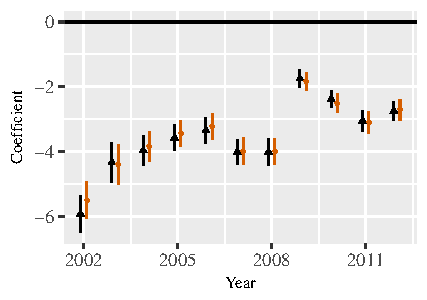
\includegraphics[height=.22\textheight, clip=true, trim=0cm .5cm 0cm .1cm]{draft_figures/rl_plots/Sum.pdf}    &
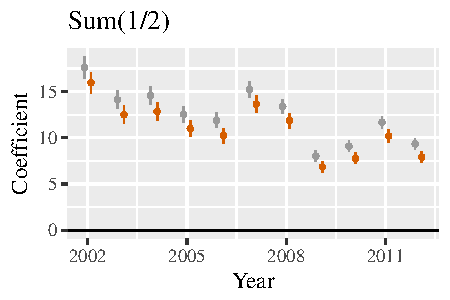
\includegraphics[height=.22\textheight, clip=true, trim=.5cm .5cm 0cm .1cm]{draft_figures/rl_plots/Sum_5.pdf}   \\
Number of Non-Zero Edges &
Lagged FDI Flow\\
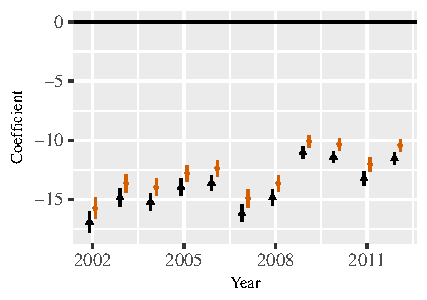
\includegraphics[height=.22\textheight, clip=true, trim=0cm .5cm 0cm .1cm]{draft_figures/rl_plots/Nonzero.pdf} &
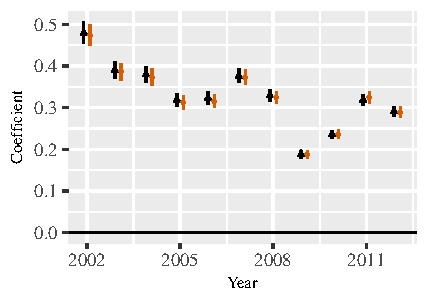
\includegraphics[height=.22\textheight, clip=true, trim=.5cm .5cm 0cm .1cm]{draft_figures/rl_plots/LDV.pdf}   \\
Log-GDP Product &
Log-Geographic Distance\\
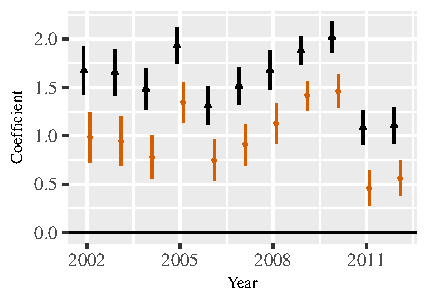
\includegraphics[height=.22\textheight, clip=true, trim=0cm .5cm 0cm .1cm]{draft_figures/rl_plots/Mass.pdf}    &
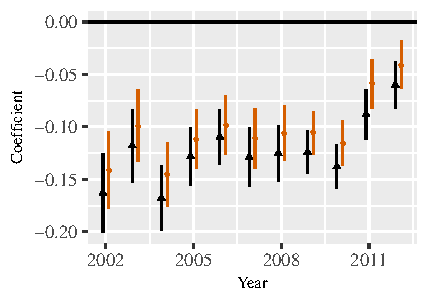
\includegraphics[height=.22\textheight, clip=true, trim=.5cm .5cm 0cm .1cm]{draft_figures/rl_plots/Distance.pdf}   \\
Contiguity &
Common Language\\
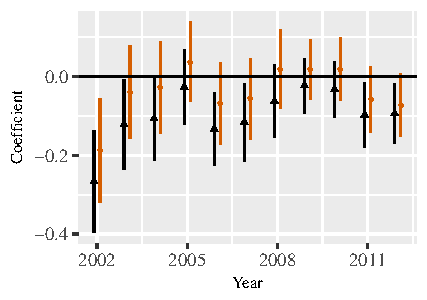
\includegraphics[height=.22\textheight, clip=true, trim=0cm .5cm 0cm .1cm]{draft_figures/rl_plots/Contiguity.pdf}  &
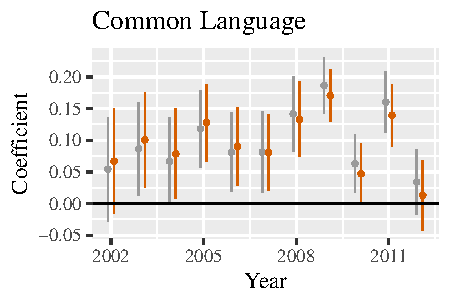
\includegraphics[height=.22\textheight, clip=true, trim=.5cm .5cm 0cm .1cm]{draft_figures/rl_plots/CommonLanguage.pdf}   \\
\end{tabular}
\caption{\label{fig:effectPlots1} Estimates of exogenous terms in Poisson ERGMs. Bars span 95\% confidence intervals. Black coefficient representations are from models excluding dependence terms (i.e., transitivity and reciprocity).}
\end{figure}




\begin{figure}[htp]
\centering
\begin{tabular}{c@{\hskip -.4cm}c}
Defense Treaty &
Non-Aggression Treaty\\
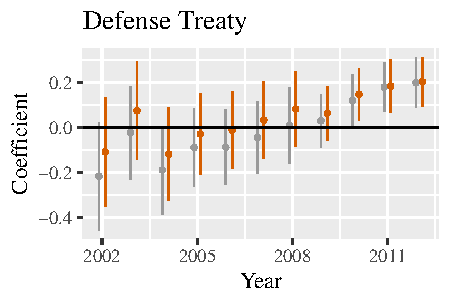
\includegraphics[height=.22\textheight, clip=true, trim=0cm .5cm 0cm .1cm]{draft_figures/rl_plots/DefenseTreaty.pdf}   &
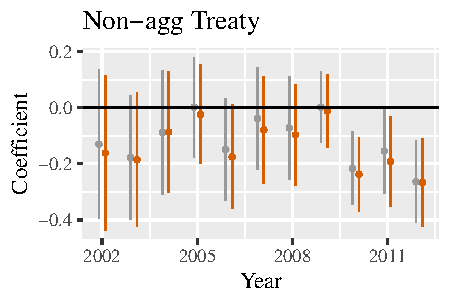
\includegraphics[height=.22\textheight, clip=true, trim=.5cm .5cm 0cm .1cm]{draft_figures/rl_plots/Non-aggTreaty.pdf}   \\
Neutrality Treaty &
Entente Treaty\\
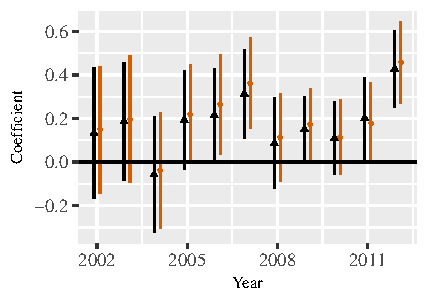
\includegraphics[height=.22\textheight, clip=true, trim=0cm .5cm 0cm .1cm]{draft_figures/rl_plots/NeutralityTreaty.pdf} &
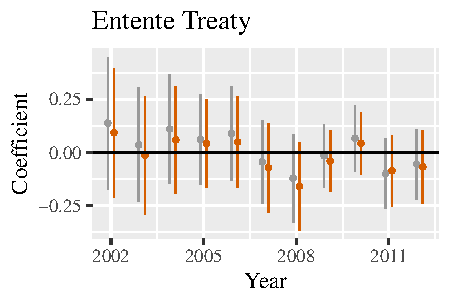
\includegraphics[height=.22\textheight, clip=true, trim=.5cm .5cm 0cm .1cm]{draft_figures/rl_plots/EntenteTreaty.pdf}   \\
PTA Depth &
Former Colony\\
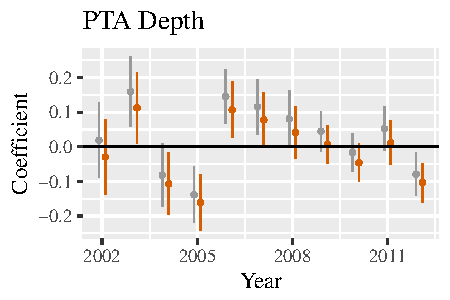
\includegraphics[height=.22\textheight, clip=true, trim=0cm .5cm 0cm .1cm]{draft_figures/rl_plots/PTADepth.pdf}    &
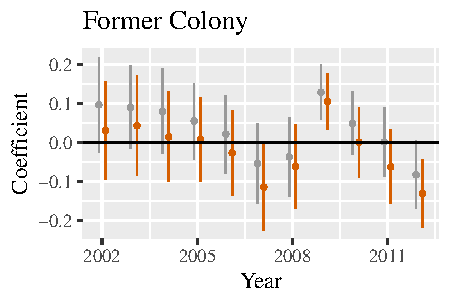
\includegraphics[height=.22\textheight, clip=true, trim=.5cm .5cm 0cm .1cm]{draft_figures/rl_plots/FormerColony.pdf}   \\
Destination GDP per capita &
Destination GDP Growth Rate\\
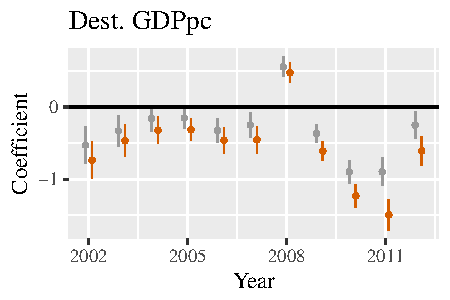
\includegraphics[height=.22\textheight, clip=true, trim=0cm .5cm 0cm .1cm]{draft_figures/rl_plots/DestGDPpc.pdf}  &
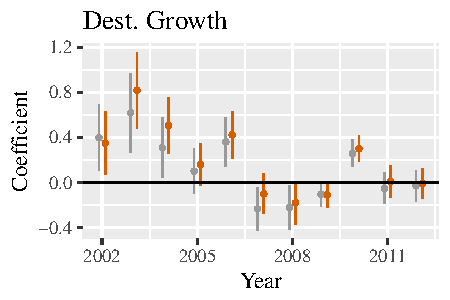
\includegraphics[height=.22\textheight, clip=true, trim=.5cm .5cm 0cm .1cm]{draft_figures/rl_plots/DestGrowth.pdf}   \\
\end{tabular}
\caption{\label{fig:effectPlots2} Estimates of exogenous terms in Poisson ERGMs. Bars span 95\% confidence intervals. Black coefficient representations are from models excluding dependence terms (i.e., transitivity and reciprocity).}
\end{figure}


\begin{figure}[htp]
\centering
\begin{tabular}{c@{\hskip -.4cm}c}
Destination Polity &
Destination Political Violence\\
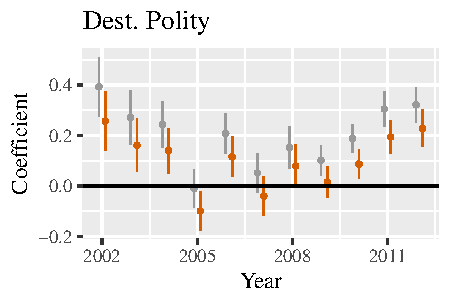
\includegraphics[height=.22\textheight, clip=true, trim=0cm .5cm 0cm .1cm]{draft_figures/rl_plots/DestPolity.pdf}    &
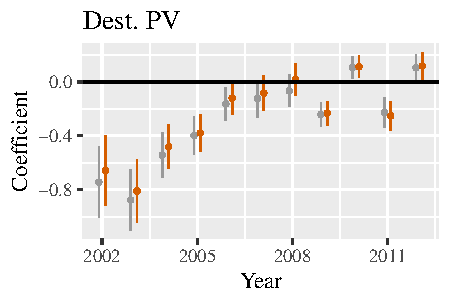
\includegraphics[height=.22\textheight, clip=true, trim=.5cm .5cm 0cm .1cm]{draft_figures/rl_plots/DestPV.pdf}   \\
Destination Trade Openness &
Origin GDP Per Capita\\
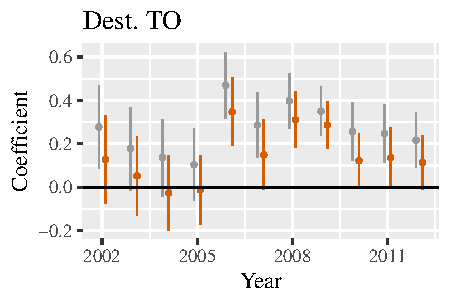
\includegraphics[height=.22\textheight, clip=true, trim=0cm .5cm 0cm .1cm]{draft_figures/rl_plots/DestTO.pdf} &
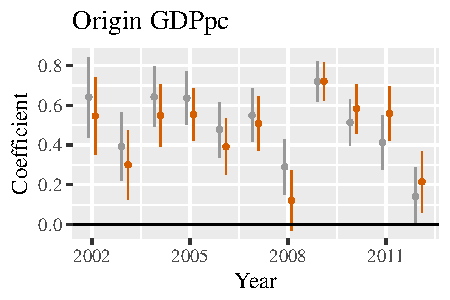
\includegraphics[height=.22\textheight, clip=true, trim=.5cm .5cm 0cm .1cm]{draft_figures/rl_plots/OriginGDPpc.pdf}   \\
Origin Growth Rate &
Origin Polity\\
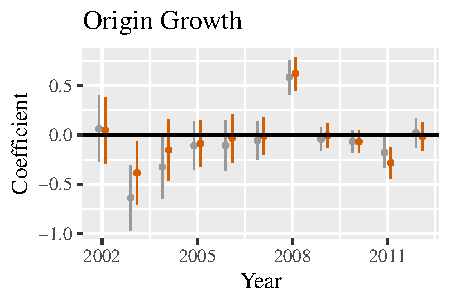
\includegraphics[height=.22\textheight, clip=true, trim=0cm .5cm 0cm .1cm]{draft_figures/rl_plots/OriginGrowth.pdf}    &
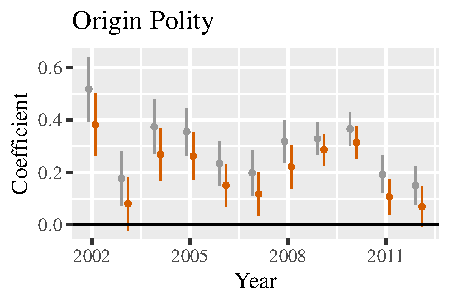
\includegraphics[height=.22\textheight, clip=true, trim=.5cm .5cm 0cm .1cm]{draft_figures/rl_plots/OriginPolity.pdf}   \\
Origin Political Violence &
Origin Trade Openness\\
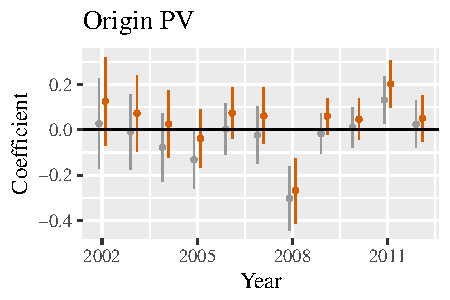
\includegraphics[height=.22\textheight, clip=true, trim=0cm .5cm 0cm .1cm]{draft_figures/rl_plots/OriginPV.pdf}  &
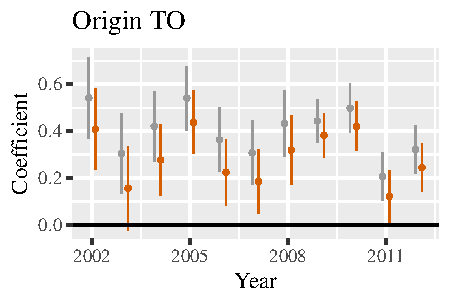
\includegraphics[height=.22\textheight, clip=true, trim=.5cm .5cm 0cm .1cm]{draft_figures/rl_plots/OriginTO.pdf}   \\
\end{tabular}
\caption{\label{fig:effectPlots3} Estimates of exogenous terms in Poisson ERGMs. Bars span 95\% confidence intervals. Black coefficient representations are from models excluding dependence terms (i.e., transitivity and reciprocity).}
\end{figure}



\begin{figure}[htp]
\centering
\begin{tabular}{c@{\hskip -.4cm}c}
Reciprocity &
Transitivity\\
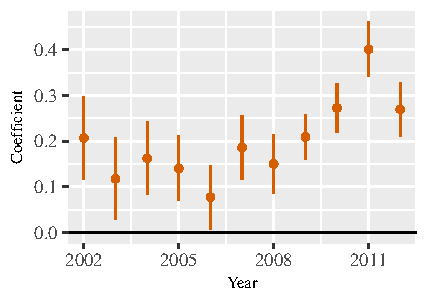
\includegraphics[height=.22\textheight, clip=true, trim=0cm .5cm 0cm .1cm]{draft_figures/rl_plots/Mutuality.pdf}    &
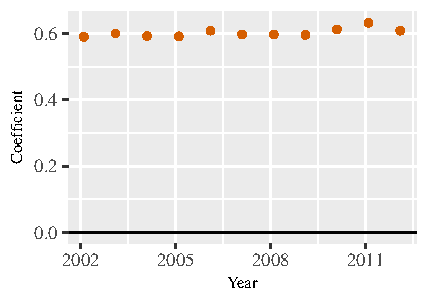
\includegraphics[height=.22\textheight, clip=true, trim=.5cm .5cm 0cm .1cm]{draft_figures/rl_plots/Transitivity.pdf}   \\
\end{tabular}
\caption{\label{fig:effectPlots4} Estimates of Network terms in Poisson ERGMs. Bars span 95\% confidence intervals.}
\end{figure}



\section{Results}

The coefficients estimated in the yearly count ERGMs are depicted in Figures \ref{fig:effectPlots1}--\ref{fig:effectPlots4}. Before discussing individual effects, we first assess the relative fit of the independence and network models. Figure \ref{fig:bic} presents the difference in Bayesian Information Criterion (BIC) in the between the independence and network models for each year in our analysis. The BIC is more conservative in terms of adding parameters to a model than the common alternative likelihood-based measure of model fit, the Akaike Information Criterion (AIC) \citep{waldorp2005model,abrahamowicz1990optimal,raftery1999bayes}. We see that the BIC in the independence model is higher than that in the network model for each year, which provides robust evidence that the network model provides a better fit to the data than the independence model over the time period that we study. Turning now to the network effects, which are presented in Figure \ref{fig:effectPlots4}, we see that the reciprocity and transitivity effects are positive and statistically significant in each year, offering robust evidence that FDI flows are interdependent according to these two canonical forms of network structure.

Interpretation

We noted above that omitting dependent network structure, a condition that characterizes previous research on FDI, can result in biased estimates and improper standard errors. For several effects that we include in our models, the results are substantively changed by adding the network parameters. In the network model, we find the following effects to be lower in magnitude, statistically significant in fewer years, or both: Gravity model mass, contiguity, PTA depth, destination polity, destination trade openness, origin trade openness, origin GDP per capita, origin polity, and origin trade openness. For each of these effects, our results indicate that omitting the network dependencies lead to either an overestimate of the effect of the respective variable, or worse, a Type 2 inferential error in which the null hypothesis of no effect is incorrectly rejected. This finding shows that, even if a researcher is not theoretically interested in network dependencies, (s)he should still incorporate them into an empirical model in order to avoid misspecification bias.

\begin{figure}[htp]
\centering
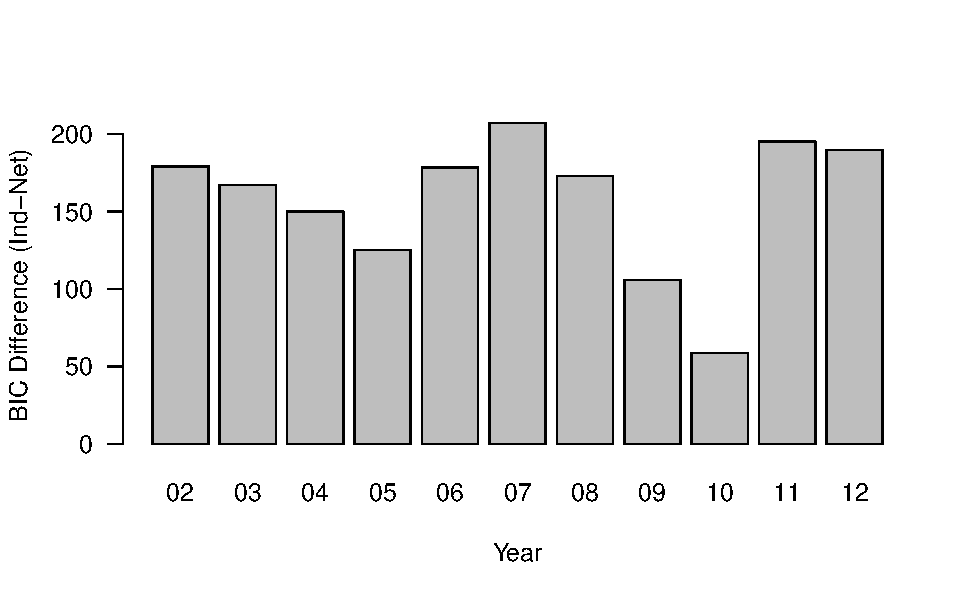
\includegraphics[scale=.75]{draft_figures/BICdiff.pdf} \vspace{-.5cm}
\caption{\label{fig:bic} Difference in BIC between independent and network model.}
\end{figure}


\section{Conclusion}
% paragraph on substantive finding

FDI flows represent ties between states that arise through both a complex underlying network of inter and intra-firm relations, and legal agreements between states. The relational backdrop through which FDI operates leads to predictable network structure in the patterns of ties formed through FDI. We present a network theory of FDI that includes reciprocity and transitivity as the core structural dependencies. The results of our statistical models confirm that these dependencies exist---a result that holds over time, and while adjusting for other covariates known to relate to FDI. This is, to our knowledge, a novel finding in the study of FDI. Our result bears important real-world implications, as network dependencies will lead to the effects of policies relevant to FDI to ripple through the network according to these dependencies.

% paragraph on methodological contribution
In addition to our substantive findings, we offer a methodological contribution to the literature on FDI. We demonstrate how the count ERGM can be used to model the effects of both covariates and network dependencies on FDI flows. We show that adding network dependencies to the covariate-based model of FDI offers a robust improvement in model fit. In future work on FDI, researchers should consider using the count ERGM, or comparable models for weighted networks. Our theory, specification, and finding of network-wide reciprocity and transitivity represent just the start in a broader scholarly dialogue on the network science of FDI flows.


\newpage
\singlespacing
\bibliographystyle{apsr}
\bibliography{fdi_reference}




\end{document}



Table \ref{tab:describe_binary} provides means for the dichotomous dyadic variables used in our models....

% Table created by stargazer v.5.2 by Marek Hlavac, Harvard University. E-mail: hlavac at fas.harvard.edu
% Date and time: Mon, Feb 20, 2017 - 22:08:59
\begin{table}[htp] \centering
  \caption{}
  \label{}
\begin{tabular}{@{\extracolsep{5pt}}lcccc}
\\[-1.8ex]\hline
\hline \\[-1.8ex]
Statistic &  \multicolumn{1}{c}{Mean} & \multicolumn{1}{c}{St. Dev.} & \multicolumn{1}{c}{Min} & \multicolumn{1}{c}{Max} \\
\hline \\[-1.8ex]
Contiguity &  0.024 & 0.152 & 0 & 1 \\
Common Official Language &  0.112 & 0.315 & 0 & 1 \\
Common Language and Ethnicity &  0.115 & 0.318 & 0 & 1 \\
Former Colonial Relationship &  0.015 & 0.121 & 0 & 1 \\
Common Colonizer &  0.062 & 0.241 & 0 & 1 \\
Defense Treaty &  0.075 & 0.264 & 0 & 1 \\
Non-aggression Treaty &  0.064 & 0.245 & 0 & 1 \\
Neutrality Treaty &  0.004 & 0.063 & 0 & 1 \\
Entente Treaty &  0.066 & 0.248 & 0 & 1 \\
\hline \\[-1.8ex]
\end{tabular}
\caption{\label{tab:describe_binary} Descriptive statistics for dichotomous dyadic covariates. Number of observations across all years is 189,000.}
\end{table}


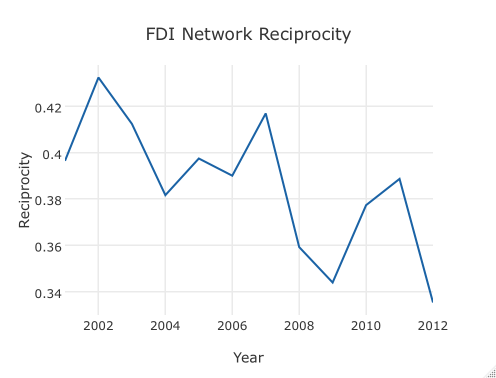
\includegraphics[scale=.8]{draft_figures/reciprocity.png}\\
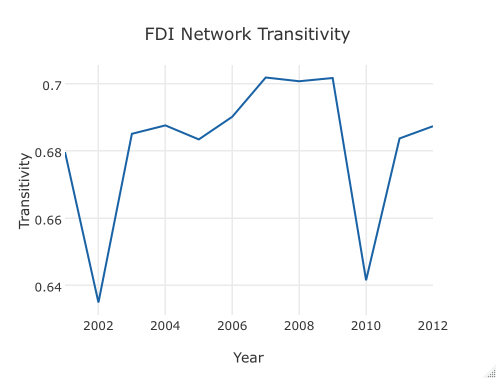
\includegraphics[scale=.8]{draft_figures/transitivity.png}\\
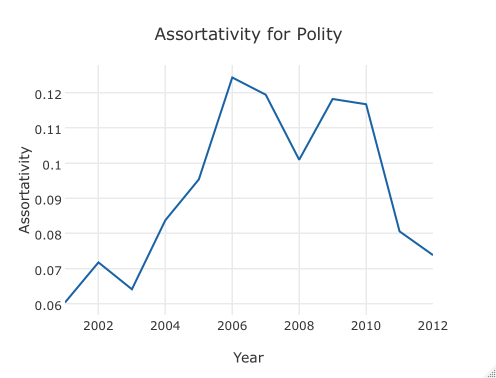
\includegraphics[scale=.8]{draft_figures/assortativity.png}\\
